\section{Ejericicio 8}

En este ejercicio se implementó la subrutina \textit{vect\_max}, la cual recibe por registros punteros a dos vectores \textit{A} y \textit{B}, los compara y devuelve en \textit{B} aquellos valores de mayor valor absoluto. 

Se reciben los punteros a los vectores A y B en los registros $r_0$ y $r_4$, respectivamente, correspondiendo  $r_0$ a una región de memoria en X, y $r_4$ a una región de memoria en Y. En el registro $n_0$ se recibe el tamaño de los vectores a comparar.
\\
\\
Se propone el siguiente \textit{main} de prueba.

\lstinputlisting[language={[Motorola68k]Assembler}]{code/ej8.asm}

En la figura~\ref{fig:ej8_results} se muestra el resultado de simular el código propuesto.

\begin{figure}[H]
    \centering
    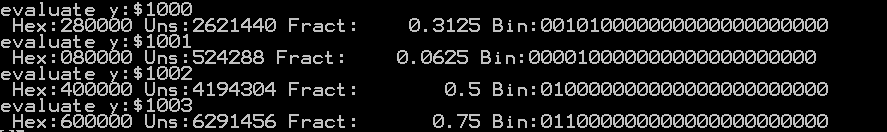
\includegraphics[width=\textwidth]{figs/ej8/ej8_result.png}
    \caption{Estado final del vector B (Simulación}.
    \label{fig:ej8_results}
\end{figure}